\documentclass{jsarticle}
\usepackage[dvipdfmx]{graphicx}
\usepackage{ascmac}
\AtBeginDocument{\RequirePackage{lmodern, times}}
\usepackage{ulem}
%%%%%%%%%%%%%%%%%
\usepackage{here}
\usepackage{txfonts}
\usepackage{listings, jlisting}
\renewcommand{\lstlistingname}{プログラム}
\lstset{language=python,
  basicstyle=\ttfamily\scriptsize,
  commentstyle=\textit,
  classoffset=1,
  keywordstyle=\bfseries,
  frame=tRBl,
  framesep=5pt,
  showstringspaces=false,
  numbers=left,
  stepnumber=1,
  numberstyle=\tiny,
  tabsize=2
}
%%%%%%%%%%%%%%%%%

\begin{document}
\title{技術資料:スピンドル冷却空気の送出系に関する計算}
\author{青木翔平}
\date{平成27年7月23日}
\maketitle

\section{スピンドル冷却系}
スピンドルの冷却に用いるシステムの構成を図\ref{fig:system}に示した.
\begin{figure}[htbp]
 \centering
 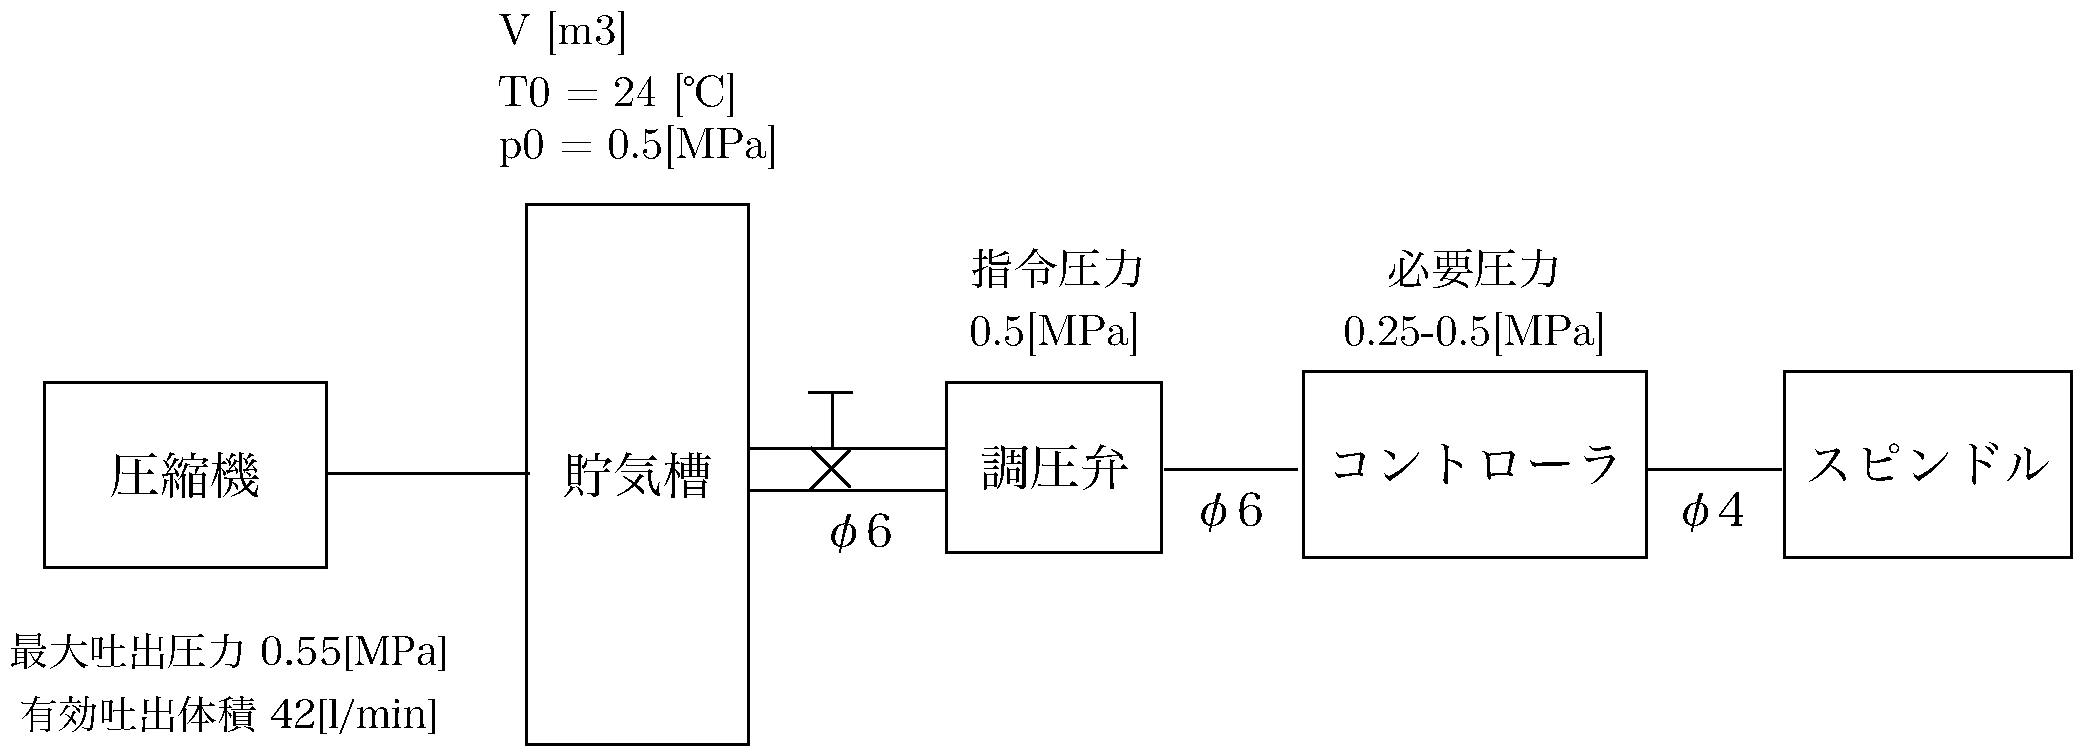
\includegraphics[width=150mm]{system.pdf}
 \caption{冷却システム構成図}
 \label{fig:system}
\end{figure}

いま,単位時間あたりに圧縮機からタンクに流入する空気質量を$\dot{m_{c}}$,タンクからスピンドルコントローラに対して流出する空気質量を$\dot{m_{c}}$とおけば,気体の状態方程式及び等エントロピー関係式から以下が成り立つ.
\begin{eqnarray}
  \dot{m_c} & = &  \frac{P\dot{V_{s1}}}{RT}  \\
  \dot{m_d} & = & \frac{p_0 A_e }{\sqrt{R T}}\sigma^{*} \label{sigma}
\end{eqnarray}


タンク内部の圧力を$p_0(t)$とおくと,流量に関する連続の式を考慮して以下が成り立つ.
\begin{eqnarray}
  p_0(t) & = & \frac{R T_0}{V} \left( m_i + \dot{m_c} dt - \dot{m_d} dt \right) \nonumber \\
  & = & \frac{R T_0}{V} \left( \frac{p_a V}{R T_0} + \frac{p_a V_{s1}}{R T_0}dt - \frac{p_0(t) A_e}{\sqrt{R T_0}} \sigma^{*} dt \right) \nonumber \\
  & = & k_3 + k_2 dt - k_1 p_0(t) dt \label{eqn:diff} 
\end{eqnarray}
ただし,
\begin{eqnarray}
  k_1 & = & \frac{\sqrt{R T_0} A_e \sigma^{*}}{V}, k_2 = p_a \frac{V_{s1}}{V}, k_3 = p_{a}
\end{eqnarray}
\sout{ $p_0(t)$を2次の項までテーラー展開して数値計算する}.
$p_0(t)$に関する差分方程式を解く.
式(\ref{eqn:diff})を微分して,
\begin{eqnarray}
  {p_0}^{\prime}(t) =  k_2 - k_1 p_0(t) 
\end{eqnarray}
が求まるから,以下の差分方程式から計算すれば良い.
\begin{eqnarray}
{p_0}(t+1) = {p_0}(t) + {p_0}^{\prime}(t) \cdot dt 
\end{eqnarray}


\begin{lstlisting}[caption=タンク内全圧の計算(main.py),label=tank_total_pressure]
from pylab import *
import numpy as np

##### BEGIN PARAMETER AREA ############
gamma = 1.4
pa = 0.1013*(10**6) #[Pa]
p0i = 5*pa #[Pa]
#CHARGE
M = 32 * 0.8 + 14 * 0.2 # O2: 80%, N2: 20%
R0 = 8.314 #(J/mol dot K)
T0 = 24 + 273.15 #[K}
R = R0/M
DISCHARGE_AIR = 42 #[l/min], ref:http://www.airbrush.co.jp/shop/products/detail.php?product_id=1296
Vs1 = DISCHARGE_AIR*0.001/60.0 #[m3/s]
#DISCHARGE
# de = 2 #[mm]
de = 1.7 #[mm]
# de = 6 #[mm]
Ae = pi*(de*0.001/2)*(de*0.001/2)#[m2]
R_kg = 289 # J/(kg dot K)
# V = 1/1000.0 #1L as [m3]
sigma = sqrt(gamma*((2/(gamma+1))**((gamma+1)/(gamma-1)))) # critical flow efficient
##### PARAMETER AREA END ############

dt = 0.01 #[sec]
tTotal = 300 #[sec]
# V = 1/1000.0 #[m3]: 1L
V_array = [1/1000.0,10/1000.0,20/1000.0,30/1000.0,40/1000.0,50/1000.0]
# V_array = [1/1000.0,20/1000.0,50/1000.0]
# V_array = [1/1000.0,50/1000.0]

# V = 1/1000.0
for V in V_array:
    pt = np.array([])
    pt = np.append(pt,p0i) 
    ts = np.array([0])
    k1 = ((R*T0)/V) * ((Ae*sigma)/(sqrt(R_kg*T0))) *1000 # x1000 is because of mass unit: kgram or gram
    # k1 = ((R*T0)/V) * ((Ae*sigma)/(sqrt(R_kg*T0))) #working bad, this is default 
    k2 = pa * Vs1 / V
    for i in xrange(int(tTotal/dt)):
        p_n = pt[-1]
        if p_n >= p0i:
            p_n_dot =  (-1.0)*k1*p_n
            p_n_dot_dot =  (-1.0)*k1*p_n_dot
            print 'compressor halted: ',i
        else:
            p_n_dot =  (-1.0)*k1*p_n + k2
            p_n_dot_dot =  (-1.0)*k1*p_n_dot
        p_n_1 = p_n + p_n_dot * dt + p_n_dot_dot*dt*dt
        pt = np.append(pt,p_n_1)
        ts = np.append(ts,dt*i)
    
    plot(ts,pt*(10**-6))

##### VISUALIZATION AREA #########
title('TANK PRESSURE TRANSITION BY AIR DISCHARGE')
legend(('1L','10L','20L','30L','40L','50L'),'upper right')
xlabel('t [sec]')
ylabel('p0 [MPa]')
ylim([0,0.6])
savefig('./image/final_pressure_depends_on_discharge_hole_size.png')
show()
\end{lstlisting}
上のプログラムは以下の様に実行する.
\begin{screen}
\$ python main.py
\end{screen}

結果を図\ref{fig:result}に示す.
\begin{figure}[htbp]
 \centering
 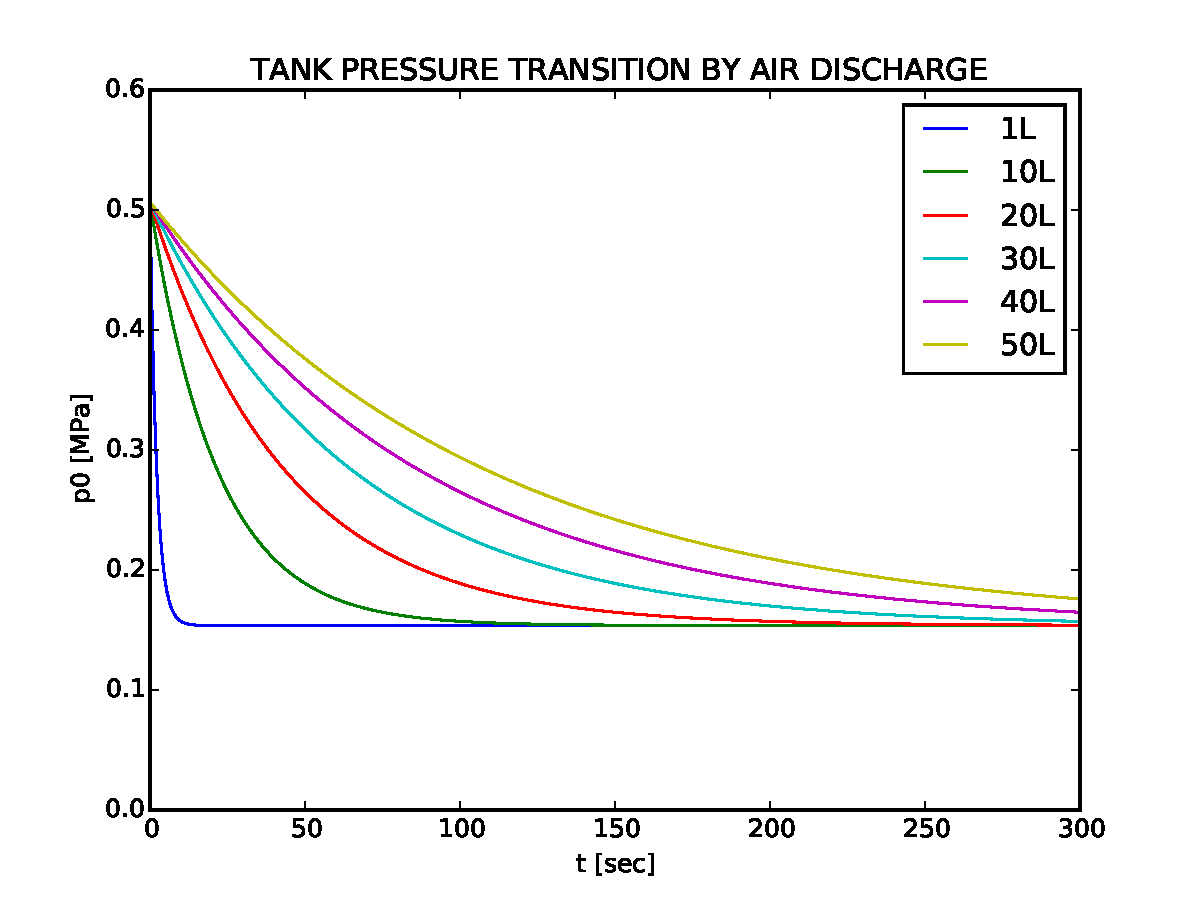
\includegraphics[width=150mm]{result.pdf}
 \caption{タンク体積に対するタンク内圧力の時間変化}
 \label{fig:result}
\end{figure}


\begin{itembox}[l]{\bf{臨界流れ係数}}
等エントロピー関係式を用いると,臨界状態(流れのマッハ数=1)となるときの圧力と全圧の関係は次式で表される.
\[
  \frac{p^{{*}}}{p_{0}}= \left( \frac{2}{\gamma+1}\right)^{\frac{\gamma}{\gamma-1}} = 0.528
\]
したがって空気(比熱比$\gamma = 1.4$)が等エントロピー的に膨張するとき,圧力が全圧の$52.8$\%まで減少したところでマッハ数=1となり,{\bf チョーク}する.
このときの流量は式(\ref{sigma})で表され,臨界流れ係数$\sigma^{*}$の大きさは
\[
\sigma^{{*}}=\sqrt {\gamma \left( \frac{2}{\gamma + 1} \right) ^{\frac{\gamma+1}{\gamma - 1}}} = 0.685
\]
である.
\end{itembox}

\section{参考資料}
[1] 松尾 一泰, 「圧縮性流体力学―内部流れの理論と解析」, オーム社, 2013

\end{document}
